
In this section, we define the fidelity and Loschmidt echo and present their corresponding spacetime path integral diagrams. It will then be evident that these quantities are just the free energy of boson with conformal interfaces (or boundaries). 

Fidelity is the square of the overlap of the groundstates of two Hamiltonians, 
\begin{equation}
{\rm fidelity} \equiv |\langle \psi_1 |\psi_2  \rangle |^2 ,
\end{equation}
For the systems we considered, $|\psi_1 \rangle$ is the groundstate of the two disconnected chains (of equal length, hence ``bipartite") and $|\psi_2\rangle$ is that of the connected chains with conformal interface. Both of them can be produced by the imaginary time evolution. Taking the horizontal axis as imaginary time, the fidelity can be diagrammatically represented as in Fig.~\ref{fig:fidel}, where the slits represents the disconnected boundary condition, such as Dirichlet(D) and Neumann(N), and the dashed line represents the conformal interface parameterized by $\lambda$. The logarithmic fidelity is then (twice) the free energy of this diagram
\begin{equation}
\mathcal{F}( {\rm fidelity} )  = - \ln \langle \psi_1 |\psi_2 \rangle^2 = - 2 \ln Z,
\end{equation}

\begin{figure}[h]
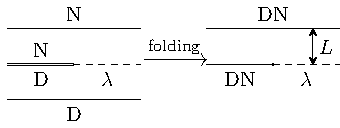
\includegraphics[width=1\columnwidth]{fig_fidelity-DN-lambda-folding.pdf}
\caption{Fidelity of connecting two CFTs. The horizontal axis is the imaginary time. Evolution along the two semi-infinite stripes produces the groundstates of the disconnected and connected chain Hamiltonians. The right diagram is the result of folding the lower part of the diagram up, so that all the boundaries are now boundary states. The solid dot represents boundary changing operator. Here D(Dirichlet), N(Neumman), $\lambda$(permeable interface parameterized by $\lambda$ are possible choices of boundary conditions.)}
\label{fig:fidel}
\end{figure}

The Loschmidt echo is also the (square of the) overlap of two wavefunctions. One of the them is the groundstate of the disconnected chains and the other is groundstate evolved by the Hamiltonian of the connected chains
\begin{equation}
\mathcal{L} \equiv |\langle \psi_{\rm gnd}  | e^{-i H t } | \psi_{\rm gnd} \rangle|^2,
\end{equation}
The path integral definition of this quantity would be similar to Fig.~\ref{fig:cut-and-join}, but to be consistent with the fidelity diagram, we take the horizontal axis as imaginary time and present it in Fig.~\ref{fig:echo}. Viewing the diagram as a partition function subject to the switching of boundary conditions, the logarithmic Loschmidt echo is also the associated free energy.

\begin{figure}[h]
\centering
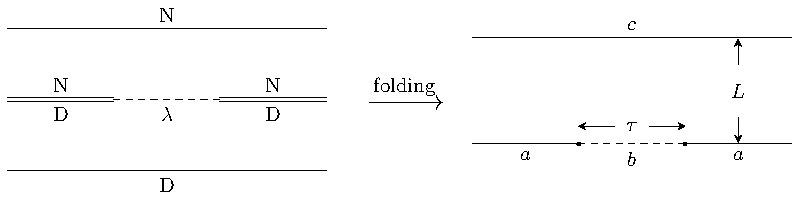
\includegraphics[width=1\columnwidth]{fig_echo-DN-lambda-folding.pdf}
\caption{Loschmidt echo of connecting two CFTs. Evolution along the two infinitely extended sides produces the groundstate of the disconnected chain Hamiltonians. They sandwich the evolution of the connected chains. In the folding picture at the right, a,b,c represent the most general boundary conditions of the chains (for example, $a$ and $c$ are DN according to the left figure). See the discussion in main text.}
\label{fig:echo}
\end{figure}

If the interface is completely transparent, i.e. at the special point of $\lambda = 1$, the tip of the slits can be regarded as corner singularities. According to Cardy and Peschel\cite{cardy_finite-size_1988}, they will contribute to a term that is logarithmic of the corner's characteristic size, which is $\ln L$ in fidelity and $\ln \tau$ in Loschmidt echo. One would expect the fidelity and echo to have power law decay with respective to these scales in the long wavelength limit. In fact, the computations have been done in Ref.~\onlinecite{stephan_logarithmic_2013,stephan_local_2011,vasseur_universal_2014,vasseur_crossover_2013,kennes_universal_2014} using either the Cardy-Peschel formula or Ward identity integration. If the slits boundary conditions are taken to be Dirichlet, we have the universal behavior for the leading term \cite{stephan_logarithmic_2013,stephan_local_2011}
\begin{equation}
\label{eq:full-pass}
\mathcal{F}({\rm fidelity}) =  \frac{c}{8} \ln L, \qquad \mathcal{F}( {\rm echo} )  = \frac{c}{4} \ln \tau .
\end{equation}

The tip of the slit is no longer a twist field with the presence of the conformal interface. Its nature is clearer in the folding picture shown in Fig.~\ref{fig:fidel} and Fig.~\ref{fig:echo} where the lower half plane is flipped up on top of the upper half plane on both fidelity and echo diagram. From the boundary conformal field theory point of view, the change of boundary condition can be regarded as insertion of primary fields called boundary condition changing (bcc) operator. These diagrams then become the one or two point functions of the bcc operators respectively, and the free energy logarithmic term extracts their scaling dimensions. 




%%% Local Variables:
%%% TeX-master: "bCFT_paper"
%%% TeX-PDF-mode: t
%%% End:
